\chapter{脂类}\label{ch:b1:lipids}

一只骆驼穿越沙漠时，驼峰里背着三十千克\omterm{def:b1:lipids:triglyceride}{脂肪}，
那里却一滴水也没有；一条生活在山涧、水温为 \qty{4}{\celsius} 的鳟鱼，
其膜的\omterm{def:b1:lipids:fluidity}{流动性}与暖池中的鲤鱼相当；把一滴橄榄油摇入水中，
它会碎成一团小液滴，
放置不动时又会重新聚成一滴。这三件事都与\omterm{def:b1:lipids:fattyacid}{脂类}有关：\omterm{def:b1:lipids:fattyacid}{脂类}是
\omterm{def:b1:organism-environment:organism}{生物体}所能携带的最致密的化学能储存库，
是包裹每个\omterm{def:b1:cell-unit-of-life:cell}{细胞}和每个\omterm{def:b1:eukaryotic-cell:organelle}{细胞器}的薄膜，
也是水拒绝溶解的一类分子。本章介绍\omterm{def:b1:lipids:fattyacid}{脂肪酸}及由其构成的\omterm{def:b1:lipids:triglyceride}{脂肪}，
能组装成膜的两亲\omterm{def:b1:lipids:fattyacid}{脂类}，
决定\omterm{def:b1:lipids:fluidity}{膜流动性}高低的因素，
以及其他\omterm{def:b1:lipids:fattyacid}{脂类}——\omterm{def:b1:lipids:amphiphilic}{固醇}、色素和激素——
它们都是由少数几个碳原子排成环或链而成的。

\section{脂肪酸}

\begin{definition}[脂类，脂肪酸]\label{def:b1:lipids:fattyacid}
\emph{脂类}\index{脂类}是由共同性质而非共同结构定义的生物分子：
它们不溶于水，而溶于非极性溶剂。
多数脂类以\emph{脂肪酸}\index{脂肪酸}为基础：
\omterm{def:b1:lipids:triglyceride}{脂肪}酸是羧酸，其烃链不分支，
含 \qtyrange{12}{24}{} 个碳原子，碳数几乎总是偶数
（它们每次以两个碳原子为单位组装，见\cref{ch:b1:biosyntheses-integration}）。
\emph{饱和脂肪酸}\index{饱和脂肪酸}只含单键，链直而柔顺；
\emph{不饱和脂肪酸}\index{不饱和脂肪酸}含有一个或多个双键，
双键为\emph{顺式}构型，每个双键使链上产生约 $30^\circ$ 的刚性折曲。
记号 C18:1 $\Delta^9$ 表示一个含 18 个碳的酸，
在第 9 位碳之后有一个双键（油酸）；
\emph{omega-3}酸的最后一个双键
位于甲基端第三个碳处。
\end{definition}

\begin{omfigure}
\begin{tikzpicture}[font=\footnotesize, line cap=round, line join=round]
  % stearic acid: zig-zag of 18 carbons
  \draw[very thick, omDef!80!black] (0,0) \foreach \i in {1,...,17} { -- ++({0.36}, {0.22*(-1)^\i}) };
  \node[fill=omThm!25, draw=omThm, rounded corners=2pt, inner sep=2pt] at (-0.1,0.0) {COOH};
  \node[anchor=east, align=right] at (-0.85,0) {硬脂酸 C18:0\\ 饱和，链直 \\ 熔点 \qty{70}{\celsius}};
  \node[anchor=west] at (6.3,-0.22) {$\mathrm{CH_3}$};
  % oleic acid: kink at carbon 9-10, second half tilted downward
  \draw[very thick, omDef!80!black] (0,-2.0) \foreach \i in {1,...,8} { -- ++({0.36}, {0.22*(-1)^\i}) };
  \draw[very thick, omDef!80!black] (2.88,-2.0) -- ++(0.36,0.22);
  \draw[double, very thick, omThm] (3.24,-1.78) -- ++(0.36,0.22);
  \draw[very thick, omDef!80!black] (3.60,-1.56) \foreach \i in {1,...,8} { -- ++({0.33}, {0.22*(-1)^(\i+1)-0.13}) };
  \node[fill=omThm!25, draw=omThm, rounded corners=2pt, inner sep=2pt] at (-0.1,-2.0) {COOH};
  \node[anchor=east, align=right] at (-0.85,-2.0) {油酸 C18:1 $\Delta^9$\\ 一个\emph{顺式}双键，折曲 \\ 熔点 \qty{13}{\celsius}};
  \node[omThm, anchor=south] at (3.42,-1.45) {\emph{顺式}双键};
  \node[anchor=west] at (6.35,-2.62) {$\mathrm{CH_3}$};
\end{tikzpicture}

{\small 两种含 18 个碳的\omterm{def:b1:lipids:fattyacid}{脂肪酸}。饱和链笔直，
与相邻分子紧密堆积；油酸中的\emph{顺式}双键使链发生折曲，
并使相邻分子保持距离，因此油酸在室温下为液体，
而硬脂酸为固体。}
\end{omfigure}

\begin{proposition}[熔点]\label{prop:b1:lipids:melting}
\omterm{def:b1:lipids:fattyacid}{脂肪酸}的熔点，以及它所属的任何\omterm{def:b1:lipids:fattyacid}{脂类}组装体的\omterm{def:b1:lipids:fluidity}{流动性}，
由链的堆积紧密程度决定：熔点随链长增加而升高
（C12:0 为 \qty{44}{\celsius}，C16:0 为 \qty{63}{\celsius}，
C18:0 为 \qty{70}{\celsius}），每增加一个\emph{顺式}双键则急剧下降
（C18:0 为 \qty{70}{\celsius}，C18:1 为 \qty{13}{\celsius}，
C18:2 为 \qty{-5}{\celsius}，C18:3 为
\qty{-11}{\celsius}）。动物\omterm{def:b1:lipids:triglyceride}{脂肪}富含饱和酸，在室温下为固体；
植物油和鱼油富含不饱和酸，
在室温下为液体。
\end{proposition}
\begin{proof}
直链彼此并排排列，每个 $\mathrm{CH_2}$ 都与相邻基团形成
范德瓦耳斯接触，每个接触约为几千焦每摩尔，
沿链累加：碳越多，接触越多，把它们分开所需的热量也越多。
折曲使链在其两侧数个碳范围内无法紧密接触，
并一次性消除许多接触。
\end{proof}

\section{脂肪：能量储存库}

\begin{definition}[甘油三酯]\label{def:b1:lipids:triglyceride}
\emph{甘油三酯}\index{甘油三酯}（三酰甘油，固态时称
\emph{脂肪}\index{脂肪}，液态时称\emph{油}\index{油}）是甘油——一种三碳醇——
的三个羟基分别与三个\omterm{def:b1:lipids:fattyacid}{脂肪酸}发生酯化反应所形成的化合物。
它不带电荷，也不含极性基团：完全疏水，
以无水液滴的形式储存于\emph{脂肪细胞}\index{脂肪细胞}中，
脂肪\omterm{def:b1:cell-unit-of-life:cell}{细胞}是脂肪\omterm{def:b1:body-plans-tissues:tissue}{组织}中的\omterm{def:b1:cell-unit-of-life:cell}{细胞}，基本上就是一滴脂肪，
其\omterm{def:b1:eukaryotic-cell:nucleus}{细胞核}被挤到
一侧。
\end{definition}

\begin{omfigure}
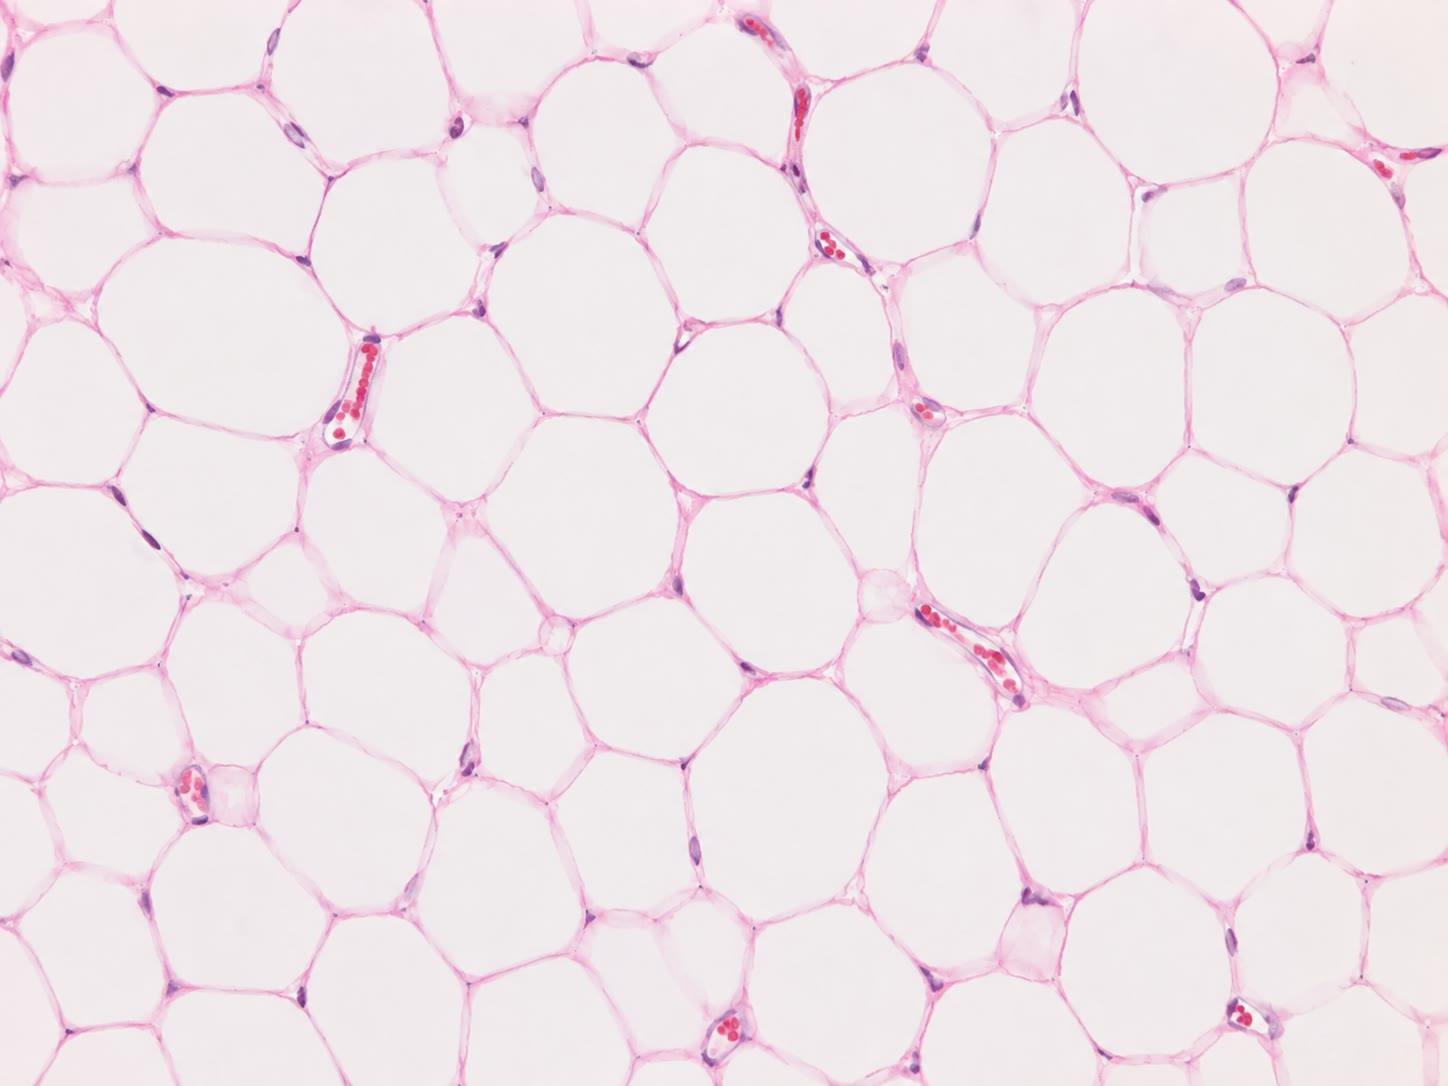
\includegraphics[width=0.5\linewidth]{images/book3/ai/b3-09-adipose-micrograph.jpg}

{\small 白色\omterm{def:b1:lipids:triglyceride}{脂肪}\omterm{def:b1:body-plans-tissues:tissue}{组织}：每个\omterm{def:b1:cell-unit-of-life:cell}{细胞}是一滴\omterm{def:b1:lipids:triglyceride}{甘油三酯}，
直径可达 \qty{100}{\micro m}，其\omterm{def:b1:cell-unit-of-life:cell}{细胞质}和\omterm{def:b1:eukaryotic-cell:nucleus}{细胞核}被挤成一圈薄边。
毛细血管穿行于\omterm{def:b1:cell-unit-of-life:cell}{细胞}之间，
负责输送和回收\omterm{def:b1:lipids:fattyacid}{脂肪酸}。}
\end{omfigure}

\begin{proposition}[脂肪是最致密的能量储存库]\label{prop:b1:lipids:energystore}
氧化 \qty{1}{g} \omterm{def:b1:lipids:triglyceride}{脂肪}释放 \qty{38}{kJ} 的能量，而 \qty{1}{g} 碳水化合物或蛋白质
仅释放 \qty{17}{kJ}：\omterm{def:b1:lipids:fattyacid}{脂肪酸}的碳原子还原程度更高
（C--H 键更多，C--O 键更少），因而向氧气转移的电子更多。此外，
\omterm{def:b1:lipids:triglyceride}{脂肪}以干燥形式储存，而糖原每克约结合 \qty{3}{g} 水：
\qty{1}{g} 储存的糖原，每克储存质量仅释放 \qty{4}{kJ}，
\omterm{def:b1:lipids:triglyceride}{脂肪}则是其九倍。一个瘦的人体内储存 \qty{0.5}{kg} 糖原
（够一天所需能量），以及
\qty{12}{kg} \omterm{def:b1:lipids:triglyceride}{脂肪}（够一个多月所需能量）。
\end{proposition}

\begin{example}[为什么不把一切都储存为脂肪]\label{ex:b1:lipids:whyglycogen}
\omterm{def:b1:lipids:triglyceride}{脂肪}只能在有氧条件下缓慢燃烧，且在动物体内不能再转化为葡萄糖
（见\cref{ch:b1:biosyntheses-integration}）；大脑和红\omterm{def:b1:cell-unit-of-life:cell}{细胞}需要葡萄糖，
而剧烈奔跑的肌肉对葡萄糖的需求速度又快于\omterm{def:b1:lipids:triglyceride}{脂肪}所能供应的速度。
糖原是快速、无需氧气的葡萄糖储存库，可供数小时之用；
\omterm{def:b1:lipids:triglyceride}{脂肪}则是致密的储存库，可供数周之用。迁徙的鸟、
冬眠的睡鼠和骆驼储存的是\omterm{def:b1:lipids:triglyceride}{脂肪}，
而短跑运动员的腿部储存的是糖原。
\end{example}

\begin{definition}[蜡]\label{def:b1:lipids:wax}
\emph{蜡}\index{蜡}是\omterm{def:b1:lipids:fattyacid}{脂肪酸}与长链
醇形成的酯：呈固态，完全疏水，用作覆层——
叶片的\omterm{def:b1:flowering-plant-organization:tissues}{角质层}（\cref{ch:b1:flowering-plant-organization}）、
昆虫体表、羽毛与皮毛的防水层，以及
蜜蜂的蜂蜡。
\end{definition}

\section{膜脂与自组装}

\begin{definition}[两亲脂质]\label{def:b1:lipids:amphiphilic}
膜脂是\emph{两亲的}\index{两亲分子}：一端为极性\emph{头部}，水能与之溶剂化；
另有一条或两条非极性\emph{尾部}，水则将其排斥。
\emph{甘油磷脂}\index{磷脂}是携带两条\omterm{def:b1:lipids:fattyacid}{脂肪酸}的甘油，
并在第三个碳上连有磷酸，磷酸再与一种小的
极性醇相连（胆碱、乙醇胺、丝氨酸、肌醇）：磷脂酰胆碱
是动物膜中最常见的脂质。\emph{鞘脂}\index{鞘脂}
以氨基醇鞘氨醇而非甘油为骨架，带有
一条\omterm{def:b1:lipids:fattyacid}{脂肪酸}，头部为磷酸胆碱（鞘磷脂）或
糖（糖脂），并富集于外小叶及
神经鞘中。\emph{固醇}\index{固醇}——动物中为\emph{胆固醇}\index{胆固醇}，
植物和真菌中则为相关固醇——是刚性的四环
分子，以单个羟基为头部，嵌于
其他脂质的尾部之间。
\end{definition}

\begin{proposition}[自组装]\label{prop:b1:lipids:selfassembly}
\index{自组装}\index{胶束}\index{脂质体}
在水中，\omterm{def:b1:lipids:amphiphilic}{两亲分子}会自发组装，以隐藏
其尾部、暴露其头部。分子的形状决定
结构：单尾脂质（\omterm{def:b1:lipids:fattyacid}{脂肪酸}、去污剂）呈
锥形，形成\emph{胶束}——直径为数纳米的球体，
尾部朝内；双尾\omterm{def:b1:lipids:amphiphilic}{磷脂}呈
圆柱形，形成\emph{双分子层}，并自身闭合为
\emph{脂\omterm{def:b1:eukaryotic-cell:plastid}{质体}}（囊泡），不留暴露的边缘。该组装
由\omterm{prop:b1:water-small-molecules:properties}{疏水效应}驱动（\cref{ch:b1:water-small-molecules}）：
它不消耗能量，也不需要酶，撕裂的双分子层会
自行重新封闭。膜是能自我修复的薄片，通过插入新
脂质而生长，绝不会凭空形成：每一张膜都来自
另一张膜。
\end{proposition}
\begin{proof}[证据]
干燥的\omterm{def:b1:lipids:amphiphilic}{磷脂}分散于水中，会形成封闭的囊泡，其
双层壁可在\omterm{prop:b1:cell-unit-of-life:microscopes}{电子显微镜}下看到（Bangham，1965）；
它们对离子和水的通透性与\omterm{def:b1:cell-unit-of-life:cell}{细胞}膜相近，
并且可以装载药物，还能与\omterm{def:b1:cell-unit-of-life:cell}{细胞}融合。加入一种
去污剂（单尾、锥形）使双分子层溶解为
混合胶束；通过透析除去去污剂，双分子层便会重新形成。
\end{proof}

\begin{omfigure}
\begin{tikzpicture}[font=\footnotesize, line cap=round]
  % micelle: ring of heads with tails pointing inward
  \foreach \a in {0,30,...,330} {
    \fill[omDef!60] ({1.2*cos(\a)},{1.2*sin(\a)}) circle (0.14);
    \draw[omDef!70!black, thick] ({1.05*cos(\a)},{1.05*sin(\a)}) -- ({0.35*cos(\a)},{0.35*sin(\a)});
  }
  \node[anchor=north, align=center] at (0,-1.55) {胶束：单尾 \\ 脂质（锥形）};
  % bilayer segment
  \foreach \i in {0,...,9} {
    \fill[omDef!60] (3.2+0.36*\i,0.75) circle (0.13); \draw[omDef!70!black, thick] (3.14+0.36*\i,0.62) -- (3.14+0.36*\i,0.1) (3.26+0.36*\i,0.62) -- (3.26+0.36*\i,0.1);
    \fill[omDef!60] (3.2+0.36*\i,-0.75) circle (0.13); \draw[omDef!70!black, thick] (3.14+0.36*\i,-0.62) -- (3.14+0.36*\i,-0.1) (3.26+0.36*\i,-0.62) -- (3.26+0.36*\i,-0.1);
  }
  \node[anchor=north, align=center] at (4.85,-1.55) {双分子层：双尾 \\ 脂质（圆柱形）};
  % liposome: two concentric rings of heads with tails between
  \foreach \a in {0,15,...,345} {
    \fill[omDef!60] ({9.3+1.45*cos(\a)},{1.45*sin(\a)}) circle (0.11);
    \draw[omDef!70!black, thick] ({9.3+1.33*cos(\a)},{1.33*sin(\a)}) -- ({9.3+1.0*cos(\a)},{1.0*sin(\a)});
    \fill[omDef!60] ({9.3+0.62*cos(\a)},{0.62*sin(\a)}) circle (0.10);
    \draw[omDef!70!black, thick] ({9.3+0.72*cos(\a)},{0.72*sin(\a)}) -- ({9.3+0.98*cos(\a)},{0.98*sin(\a)});
  }
  \node at (9.3,0) {水};
  \node[anchor=north, align=center] at (9.3,-1.55) {脂质体：自身闭合的 \\ 双分子层，无边缘};
\end{tikzpicture}

{\small 两亲脂质在水中的三种组装。锥形的
单尾分子堆积成胶束；圆柱形的双尾\omterm{def:b1:lipids:amphiphilic}{磷脂}
形成双分子层，并闭合为囊泡以隐藏其
边缘。}
\end{omfigure}

\begin{omfigure}
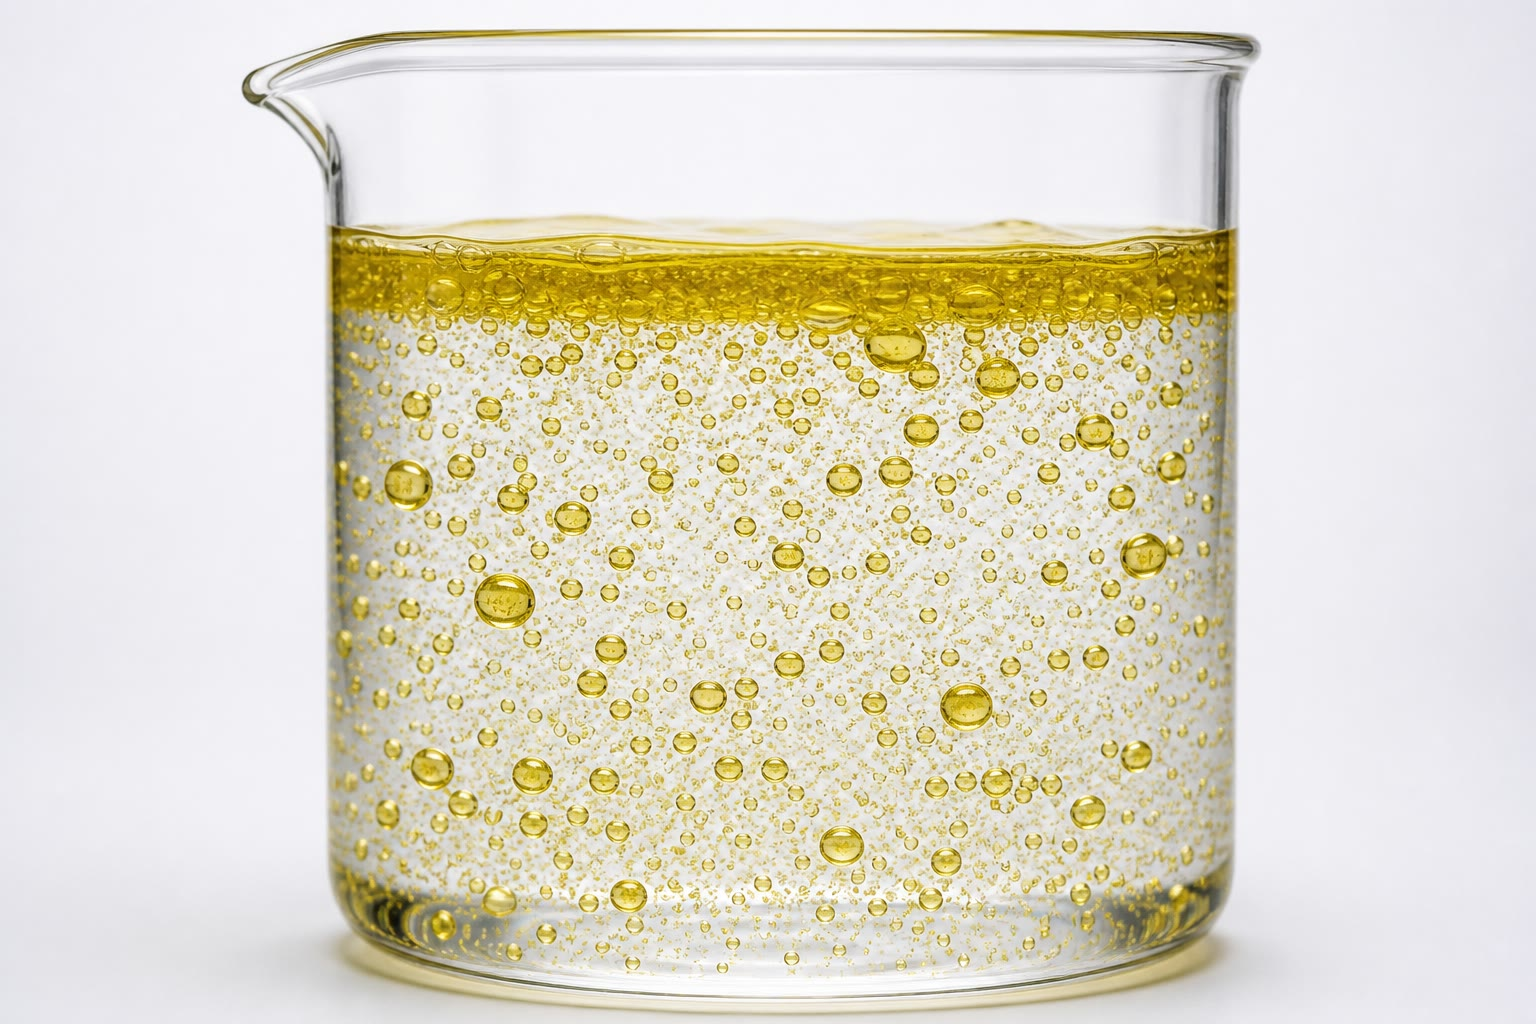
\includegraphics[width=0.5\linewidth]{images/book3/ai/b3-09-oil-water-emulsion.jpg}

{\small 油被摇入水中：形成一团液滴云，若无
两亲物质——去污剂、胆汁盐、\omterm{def:b1:lipids:amphiphilic}{磷脂}——包裹
它们，数分钟内便会聚并。乳化作用正是消化道
在酶够得着膳食\omterm{def:b1:lipids:triglyceride}{脂肪}之前对其所做的处理。}
\end{omfigure}

\begin{example}[胆汁盐]\label{ex:b1:lipids:bile}
膳食\omterm{def:b1:lipids:triglyceride}{脂肪}以油的形式进入肠道；消化\omterm{def:b1:lipids:triglyceride}{脂肪}的\omterm{def:b1:lipids:triglyceride}{脂肪}酶
只在油–水界面起作用。胆汁盐是
\omterm{def:b1:lipids:amphiphilic}{胆固醇}的两亲衍生物，将\omterm{def:b1:lipids:triglyceride}{脂肪}包裹成直径约一微米的液滴，
使界面面积增大千倍，随后又把释放出的\omterm{def:b1:lipids:fattyacid}{脂肪酸}以胶束的形式
运送至吸收\omterm{def:b1:cell-unit-of-life:cell}{细胞}
（\cref{ch:b1:digestion-absorption}）。肥皂也利用同样的原理。
\end{example}

\section{膜的流动性}

\begin{definition}[流动性，相变]\label{def:b1:lipids:fluidity}
\omterm{def:b1:membranes-transport:membrane}{脂双层}具有一个\emph{相变温度}\index{相变温度} $T_m$：低于该温度时，链排列
有序，呈凝胶状，脂质几乎不移动；高于该温度时，链变得无序，
双分子层成为二维流体，其中的脂质每秒钟与邻居互换位置上百万次，
并以\qty{1}{\micro m/s}的速度
穿过膜面。\omterm{def:b1:cell-unit-of-life:cell}{细胞}使其膜保持在
$T_m$ 之上：\emph{流动性}\index{膜流动性}使蛋白质得以
扩散和旋转，囊泡得以出芽与融合，双分子层也能重新封闭。
\end{definition}

\begin{proposition}[决定流动性的因素]\label{prop:b1:lipids:fluidityfactors}
$T_m$ 随链长增加而升高，随不饱和程度增加而降低，
游离\omterm{def:b1:lipids:fattyacid}{脂肪酸}的情况与此相同；由 C18:0 链构成的双分子层
在 \qty{55}{\celsius} 熔化，由 C18:1 链构成的则在 \qty{-20}{\celsius} 熔化。
\omterm{def:b1:lipids:amphiphilic}{胆固醇}插入尾部之间，具有双重作用：在
$T_m$ 以上，其刚性环限制链的运动，使膜变硬；
在 $T_m$ 以下，其刚性环阻止链紧密堆积，
从而防止膜凝固。它使相变展宽为渐变过程，并
在较宽的温度范围内使\omterm{def:b1:lipids:fluidity}{流动性}基本保持恒定——
相当于\omterm{def:b1:lipids:fluidity}{流动性}的缓冲器。动物\omterm{def:b1:membranes-transport:membrane}{质膜}中，\omterm{def:b1:lipids:amphiphilic}{胆固醇}与\omterm{def:b1:lipids:amphiphilic}{磷脂}的比例最高可达
1:1，即每个\omterm{def:b1:lipids:amphiphilic}{磷脂}对应一个\omterm{def:b1:lipids:amphiphilic}{胆固醇}。
\end{proposition}

\begin{omfigure}
\begin{tikzpicture}
\begin{axis}[
  width=0.86\linewidth, height=6.0cm,
  axis x line=bottom, axis y line=left,
  xmin=-20, xmax=60, ymin=0, ymax=1.15,
  xlabel={温度 (\unit{\celsius})}, ylabel={流动性（相对值）},
  xlabel style={font=\small, at={(axis description cs:0.5,-0.12)}, anchor=north},
  ylabel style={font=\small},
  tick label style={font=\small}, xtick={-20,0,20,40,60}, ytick={0,0.5,1},
  legend style={font=\small, at={(0.03,0.97)}, anchor=north west, draw=none},
  clip=false,
]
\addplot[very thick, omDef, domain=-20:60, samples=120] {1/(1+exp(-(x-41)/1.5))};
\addlegendentry{饱和 C16 链，无胆固醇}
\addplot[very thick, omProp, domain=-20:60, samples=120] {1/(1+exp(-(x+5)/1.5))};
\addlegendentry{每个脂质含一个 \emph{cis} 双键}
\addplot[very thick, omThm, domain=-20:60, samples=120] {0.15+0.7/(1+exp(-(x-20)/12))};
\addlegendentry{饱和链，含 \qty{30}{\%} 胆固醇}
\draw[dashed, gray] (axis cs:37,0) -- (axis cs:37,1.05);
\node[font=\scriptsize, anchor=south] at (axis cs:37,1.06) {\qty{37}{\celsius}};
\end{axis}
\end{tikzpicture}

{\small 三种双分子层的\omterm{def:b1:lipids:fluidity}{流动性}随温度的变化。饱和链
在 \qty{40}{\celsius} 附近急剧凝固；每个脂质含一个双键，
使\omterm{def:b1:lipids:fluidity}{相变温度}降至零度以下；\omterm{def:b1:lipids:amphiphilic}{胆固醇}使相变变为平缓的斜坡，
使膜在生理温度范围内既不呈固态，
也不过于流动。}
\end{omfigure}

\begin{proposition}[同型黏度适应]\label{prop:b1:lipids:homeoviscous}
\index{同型黏度适应}
无法调节自身温度的生物通过调整膜的组成
来保持\omterm{def:b1:lipids:fluidity}{流动性}恒定：温度降低时，
它们以\omterm{def:b1:lipids:fattyacid}{不饱和脂肪酸}替代\omterm{def:b1:lipids:fattyacid}{饱和脂肪酸}，
以较短的链替代较长的链；温度升高时则相反。
\end{proposition}
\begin{proof}[证据]
\emph{E. coli} 在 \qty{10}{\celsius} 下培养时，\omterm{def:b1:lipids:fattyacid}{不饱和脂肪酸}的比例
是同一菌株在 \qty{40}{\celsius} 下培养时的两倍；
两种培养物的膜，以探针的迁移率测得，
在各自的生长温度下\omterm{def:b1:lipids:fluidity}{流动性}相同。鳟鱼
适应 \qty{5}{\celsius} 的鳟鱼，其膜脂中的多\omterm{def:b1:lipids:fattyacid}{不饱和脂肪酸}
比 \qty{20}{\celsius} 下的鳟鱼更多；
靠近雪地的驯鹿腿部\omterm{def:b1:lipids:triglyceride}{脂肪}，
比躯干部位的\omterm{def:b1:lipids:triglyceride}{脂肪}更不饱和。能够耐受霜冻的植物
在秋季增加膜中不饱和脂质的含量，而无法这样做的突变体
在受冷时死亡。
\end{proof}

\begin{example}[黄油、橄榄油与鱼油]\label{ex:b1:lipids:kitchen}
黄油（\qty{65}{\%} 为饱和\omterm{def:b1:lipids:triglyceride}{脂肪}）在冰箱中呈固态，
在室温下变软；橄榄油（\qty{75}{\%} 为油酸）在室温下呈液态，
放入冰箱后会变浑浊；鱼油富含
五个和六个双键的 omega-3 酸，在
\qty{-20}{\celsius} 下仍保持液态，这正是北大西洋中
鳕鱼的膜所需要的性质。
\end{example}

\section{固醇、色素与信号}

\begin{definition}[类固醇、类异戊二烯]\label{def:b1:lipids:steroids}
\emph{类固醇}\index{类固醇}具有与\omterm{def:b1:lipids:amphiphilic}{胆固醇}相同的四个稠合环：
\omterm{def:b1:lipids:amphiphilic}{胆固醇}本身（构成膜，也是其余类\omterm{def:b1:lipids:amphiphilic}{固醇}的前体）、胆汁盐、
维生素 D，以及类\omterm{def:b1:lipids:amphiphilic}{固醇}激素——皮质醇、醛固酮、
性激素——这些都是小分子、疏水分子，能自由穿过膜，
并作用于\omterm{def:b1:cell-unit-of-life:cell}{细胞}内的受体。\emph{类异戊二烯}\index{类异戊二烯}
（萜类）是由五碳异戊二烯单元组成的链与环：
\emph{类胡萝卜素}使胡萝卜呈色并保护\omterm{def:b1:eukaryotic-cell:plastid}{叶绿体}
（见\cref{ch:b1:photosynthesis}）、叶绿素的侧链、
电子传递链中的醌类、橡胶，以及脂溶性
维生素 A、E 和 K。
\end{definition}

\begin{proposition}[脂质的功能]\label{prop:b1:lipids:functions}
能量储存（\omterm{def:b1:lipids:triglyceride}{甘油三酯}）；构成膜（\omterm{def:b1:lipids:amphiphilic}{磷脂}、\omterm{def:b1:lipids:amphiphilic}{鞘脂}、
\omterm{def:b1:lipids:amphiphilic}{固醇}）；绝缘与防水（\omterm{def:b1:lipids:triglyceride}{脂肪}、蜡）；光吸收
与保护（类胡萝卜素）；电子传递（醌类）；信号传递
在\omterm{def:b1:cell-unit-of-life:cell}{细胞}之间（\omterm{def:b1:lipids:steroids}{类固醇}激素、前列腺素）及\omterm{def:b1:cell-unit-of-life:cell}{细胞}内部
（肌醇\omterm{def:b1:lipids:amphiphilic}{磷脂}、二酰甘油）；维生素。一个性质——
不溶于水——是上述所有功能的基础：脂质停留在所放之处，
无论是油滴、薄膜还是膜，或是
不借助载体穿过膜。
\end{proposition}

\begin{example}[不需要表面受体的激素]\label{ex:b1:lipids:steroidhormone}
皮质醇由肾上腺分泌，在血液中与
\omterm{def:b1:membranes-transport:transporters}{载体蛋白}结合运输；到达靶\omterm{def:b1:cell-unit-of-life:cell}{细胞}后离开载体，
数秒内即可溶解穿过\omterm{def:b1:membranes-transport:membrane}{质膜}，并与\omterm{def:b1:eukaryotic-cell:organelle}{细胞溶胶}中的受体结合，
该复合物随后进入\omterm{def:b1:eukaryotic-cell:nucleus}{细胞核}，开启基因
（见\cref{ch:b1:expression-control}）。蛋白质类激素如胰岛素，
能溶于水，分子又太大，无法穿过膜，必须在\omterm{def:b1:cell-unit-of-life:cell}{细胞}外与受体结合，
再将信息传入\omterm{def:b1:cell-unit-of-life:cell}{细胞}内。信使的化学性质
决定了信息的传递途径。
\end{example}

\section{练习}

\begin{exercise}[$\star$]\label{exo:b1:lipids:1}
给出脂质的定义，并说明为什么
该定义依据的是性质而不是结构。
\end{exercise}

\begin{exercise}[$\star$]\label{exo:b1:lipids:2}
写出亚油酸的记号（18 个碳，双键在
第 9 与第 12 位碳之后），并判断它是 omega-3 酸还是 omega-6 酸。
\end{exercise}

\begin{exercise}[$\star$]\label{exo:b1:lipids:3}
为什么\omterm{def:b1:lipids:triglyceride}{甘油三酯}形成液滴，而\omterm{def:b1:lipids:amphiphilic}{磷脂}
形成\omterm{def:b1:membranes-transport:membrane}{脂双层}？造成这一差别的结构原因是什么？
\end{exercise}

\begin{exercise}[$\star$]\label{exo:b1:lipids:4}
由\omterm{def:b1:lipids:fluidity}{流动性}图可知，三种\omterm{def:b1:membranes-transport:membrane}{脂双层}各自
处于相变中点时的温度分别为多少？若某细菌生活在
\qty{10}{\celsius} \omterm{def:b1:organism-environment:organism}{环境}中，你预计其中哪一种\omterm{def:b1:membranes-transport:membrane}{脂双层}会出现在该细菌中？
\end{exercise}

\begin{exercise}[$\star\star$]\label{exo:b1:lipids:5}
一个人储存了 \qty{15}{kg} \omterm{def:b1:lipids:triglyceride}{脂肪}。计算其所含的能量，
能维持的天数（每日静息消耗为
\qty{8}{MJ/d}），以及储存同等能量所需的
水合糖原质量。
\end{exercise}

\begin{exercise}[$\star\star$]\label{exo:b1:lipids:6}
按熔点对 C14:0、C18:0、C18:1、C18:3、C22:0 进行排序，并
说明排序中每一步的理由。
\end{exercise}

\begin{exercise}[$\star\star$]\label{exo:b1:lipids:7}
一个红\omterm{def:b1:cell-unit-of-life:cell}{细胞}的表面积为 \qty{140}{\micro m^2}；一个\omterm{def:b1:lipids:amphiphilic}{磷脂}
头部占据 \qty{0.6}{nm^2}。计算膜（两层）中的\omterm{def:b1:lipids:amphiphilic}{磷脂}分子数，
并在 \qty{750}{g/mol} 下计算它们的
总质量（以皮克为单位）。
\end{exercise}

\begin{exercise}[$\star\star$]\label{exo:b1:lipids:8}
\qty{1}{g} 橄榄油（密度为 \qty{0.9}{g/mL}）被乳化成
直径为 \qty{1}{\micro m} 的液滴。计算总界面
面积；对单个液滴重复计算。为什么胰\omterm{def:b1:lipids:triglyceride}{脂肪}酶需要
乳液？
\end{exercise}

\begin{exercise}[$\star\star$]\label{exo:b1:lipids:9}
说明\omterm{def:b1:lipids:amphiphilic}{胆固醇}对\omterm{def:b1:lipids:fluidity}{膜流动性}的两种相反作用，
以及为什么含\omterm{def:b1:lipids:amphiphilic}{胆固醇}的膜不存在明显的相变。
\end{exercise}

\begin{exercise}[$\star\star\star$]\label{exo:b1:lipids:10}
一株突变植物不能合成\omterm{def:b1:lipids:fattyacid}{不饱和脂肪酸}。预测其膜在
\qty{25}{\celsius} 和 \qty{5}{\celsius} 时的状态，
以及寒冷的夜晚其\omterm{def:b1:cell-unit-of-life:cell}{细胞}会发生什么，野生型为何能存活。
\end{exercise}

\begin{exercise}[$\star\star\star$]\label{exo:b1:lipids:11}
每克被氧化的\omterm{def:b1:lipids:triglyceride}{脂肪}产生 \qty{1.07}{g} 水（糖原
为 \qty{0.56}{g}，蛋白质为 \qty{0.4}{g}）。计算一头骆驼
氧化 \qty{1}{kg} \omterm{def:b1:lipids:triglyceride}{脂肪}所产生的水。所需氧气为每克\omterm{def:b1:lipids:triglyceride}{脂肪}
\qty{2}{L}；以干燥沙漠空气呼吸时，
每升通入的空气约损失 \qty{0.03}{g} 水，氧提取率为 \qty{5}{\%}。
计算呼吸损失的水量，并判断
驼峰是否为水的储备。
\end{exercise}

\begin{exercise}[$\star\star\star$]\label{exo:b1:lipids:12}
“膜能够自组装，但\omterm{def:b1:cell-unit-of-life:cell}{细胞}不能从无到有
制造膜。”请用一段话调和这句话的两半，
运用\omterm{prop:b1:water-small-molecules:properties}{疏水效应}、膜通过插入而生长，以及
膜在\omterm{def:b1:cell-unit-of-life:cell}{细胞}分裂中的连续性。
\end{exercise}

\section{问题：冷水与沙漠脂肪}

\begin{problem}[{周末问题——山溪中鳟鱼的膜与沙漠中骆驼的驼峰，
不饱和度、相变温度，
能量密度与代谢水，
以储存脂肪代替糖原所节省的质量为结尾}]
\label{pb:b1:lipids:1}
第一部分涉及一条鳟鱼，其膜\omterm{def:b1:lipids:amphiphilic}{磷脂}的\omterm{def:b1:lipids:fattyacid}{脂肪酸}链为
C16:0、C18:1 和 C22:6（一种含六个双键的 omega-3 酸）。第二部分
涉及一头体重 \qty{500}{kg} 的单峰驼，其驼峰中含有
\qty{30}{kg} \omterm{def:b1:lipids:triglyceride}{甘油三酯}，它穿越沙漠时的\omterm{def:b1:organism-environment:allometry}{代谢率}为
\qty{60}{MJ/d}。能量：\omterm{def:b1:lipids:triglyceride}{脂肪} \qty{38}{kJ/g}，糖原 \qty{17}{kJ/g}
（干重），储存时每克伴有 \qty{3}{g} 水。代谢水：
每克\omterm{def:b1:lipids:triglyceride}{脂肪}产水 \qty{1.07}{g/g}。氧气：每克\omterm{def:b1:lipids:triglyceride}{脂肪}需 \qty{2.0}{L}；空气
中氧含量为 \qty{21}{\%}，骆驼只提取其吸入氧气的 \qty{5}{\%}，
呼出空气比
吸入的沙漠空气多携带 \qty{30}{g/m^3} 水。

\medskip
\noindent\textbf{第一部分——鳟鱼。}
适应 \qty{20}{\celsius} 的鳟鱼，其膜中\omterm{def:b1:lipids:fattyacid}{脂肪酸}链的组成为
\qty{40}{\%} C16:0、\qty{45}{\%} C18:1 和 \qty{15}{\%} C22:6；在
\qty{5}{\celsius} 时的鳟鱼则分别为 \qty{25}{\%}、\qty{40}{\%} 和 \qty{35}{\%}。
\begin{enumerate}
  \item 写出三种酸的记号，并数出每种酸的
        每条链中的双键数。
  \item 计算每个温度下每条链
        的平均双键数。
  \item 从链的堆积角度说明，这一变化为何会降低
        膜的\omterm{def:b1:lipids:fluidity}{相变温度}。
  \item \omterm{def:b1:membranes-transport:membrane}{脂双层}的 $T_m$ 约下降 \qty{20}{\celsius}，
        即每条链平均每增加 \qty{0.5}{} 个双键。估算
        两条鳟鱼之间 $T_m$ 的变化量。
  \item 温水鳟鱼的膜在 \qty{20}{\celsius} 时呈流动态，但
        在 \qty{5}{\celsius} 时会凝胶化。若遇突然的寒夜，
        其转运蛋白、泵和神经传导会
        发生什么变化？
  \item 这种适应需要数天。写出鳟鱼必须多合成的
        哪些酶，并说明它们在\omterm{def:b1:cell-unit-of-life:cell}{细胞}的何处发挥作用（见\cref{ch:b1:eukaryotic-cell}）。
  \item 两条鳟鱼的膜中，\omterm{def:b1:lipids:amphiphilic}{胆固醇}与\omterm{def:b1:lipids:amphiphilic}{磷脂}的比例均为
        一个\omterm{def:b1:lipids:amphiphilic}{胆固醇}分子对两个\omterm{def:b1:lipids:amphiphilic}{磷脂}分子。说明\omterm{def:b1:lipids:amphiphilic}{胆固醇}在两种情况下各起什么作用。
\end{enumerate}

\medskip
\noindent\textbf{第二部分——骆驼的能量。}
\begin{enumerate}[resume]
  \item 计算驼峰中储存的能量。
  \item 这些能量可维持穿越过程的多少天？
  \item 计算储存相同能量所需的干糖原质量，
        以及含水糖原的质量。
  \item 计算以\omterm{def:b1:lipids:triglyceride}{脂肪}而非糖原储存能量所节省的质量，
        并将其表示为骆驼体重的分数。
  \item \omterm{def:b1:lipids:triglyceride}{脂肪}储存于驼峰中，而非分散在皮下。
        依据
        \cref{ch:b1:mammal-organization}中的热量收支，提出一个理由。
\end{enumerate}

\medskip
\noindent\textbf{第三部分——驼峰是否为水的储存库？}
\begin{enumerate}[resume]
  \item 计算氧化整个
        驼峰所产生的代谢水。
  \item 计算所需氧气的体积（以升计）。
  \item 计算骆驼为获得上述氧气必须通气的
        空气体积。
  \item 计算呼出该空气时失去的水分。
  \item 比较获得的水与失去的水，并作出结论。
  \item 骆驼不靠出汗，而是让体温在白天升高
        \qty{6}{\celsius}，夜间降温。计算
        它以此方式储存的热量（热容
        \qty{3.5}{kJ.kg^{-1}.K^{-1}}）以及蒸发
        同等热量所需的水量（\qty{2.4}{kJ/g}）。
  \item 骆驼可失去 \qty{25}{\%} 的体内水分而存活，
        其红\omterm{def:b1:cell-unit-of-life:cell}{细胞}可膨胀至原体积的两倍而不破裂，
        当其在十分钟内饮水 \qty{100}{L} 时。
        请将后一性质与\cref{ch:b1:membranes-transport}中的膜联系起来。
\end{enumerate}

\medskip
\noindent\textbf{第四部分——双层膜的计算。}
一个\omterm{def:b1:lipids:amphiphilic}{磷脂}头部占据 \qty{0.65}{nm^2} 的面积；双层膜
厚 \qty{5}{nm}；骆驼红\omterm{def:b1:cell-unit-of-life:cell}{细胞}的表面积为
\qty{80}{\micro m^2}，每升血液中含 $\num{8e12}$ 个红\omterm{def:b1:cell-unit-of-life:cell}{细胞}。
\begin{enumerate}[resume]
  \item 计算一个红\omterm{def:b1:cell-unit-of-life:cell}{细胞}膜中\omterm{def:b1:lipids:amphiphilic}{磷脂}分子的数目。
  \item 计算 \qty{40}{L} 血液中全部红\omterm{def:b1:cell-unit-of-life:cell}{细胞}所含\omterm{def:b1:lipids:amphiphilic}{磷脂}分子的数目。
  \item 取摩尔质量为 \qty{750}{g/mol}，计算该脂质的质量（以克计）。
  \item \omterm{def:b1:lipids:amphiphilic}{磷脂}分子从膜的一层翻转到另一层的
        过程自发发生，约每周一次，而其侧向扩散
        在一秒内可达 \qty{1}{\micro m}。试从
        \omterm{prop:b1:water-small-molecules:properties}{疏水效应}解释这两个数值。
  \item 结合翻转速率，解释为何膜的两层
        在\omterm{def:b1:cell-unit-of-life:cell}{细胞}的整个生命周期内
        可保持组成不同。
  \item 给出结果：骆驼以携带
        \qty{30}{kg} \omterm{def:b1:lipids:triglyceride}{脂肪}而非等能量糖原所节省的质量，
        以及对驼峰作为水储存库的结论。
\end{enumerate}
\end{problem}
